The lepton charge mis-measurement commonly referred to as ``charge flip'', 
is an experimental background strongly associated to analyses relying on same-sign lepton final states. 
In those events, the electric charge of one of the two leptons forming an opposite-sign (OS) pair, 
coming from an abundant SM process ($pp\to Z$, \ttbar, $W^+W^-$\ldots), 
is mis-identified leading to a much rarer same-sign (SS) pair event.
In most cases, the source of such a mis-identification 
is the creation of additional close-by tracks $e^\pm\to e^\pm\gamma\to e^\pm e^\pm e^\mp$ 
via Brehmstrahlung of the original electron when interacting with the material of the inner tracker. 
If one of the secondary electron tracks is subsequently preferred to the original track in the reconstruction of the electron candidate, 
the charge assigned to the electron might be incorrect, leading to a charge-flip event. 
Errors on the track charge assignment itself may occur as well, but they are much rarer. 
In the case of muons, charge-flip is essentially negligible due to the much smaller interaction cross-section with matter, 
and the requirement of identical charges to be measured for the inner tracker and muon spectrometer tracks. 

A purely data-driven method is used to estimate event yields for the 
electron charge-flip background. 
Assuming that the electron charge flip rates $\xi(\eta,\pt)$ are known, 
a simple way to predict these yields is to select events with pairs of opposite-sign leptons in data and assign them a weight:

\begin{align}
w_\text{flip} = \xi_1(1-\xi_2) + (1-\xi_1)\xi_2
\label{eqn:chargeflip_weight}
\end{align}
where $\xi_{(i)}=0$ for muons.

The advantages of this method are a good statistical precision since the charge flip rate is quite small, 
and the absence of dependency to the simulation and related uncertainties. 
Obviously, it requires a precise measurement of the rates, which is described in this section. 
An inconvenience of this approach is that the reconstructed momentum for charge-flipped electrons  
tends to be negatively biased (too low by a few GeV), 
since such important Brehmstrahlung topologies represent only 
a very small fraction of the cases used to tune electron energy calibration. 
Simply re-weighting electrons from opposite-sign lepton pairs therefore does not predict correctly 
the charge-flip background shape for variables very sensitive to the electron momentum, for example the $m_{ee}$ line-shape. 
However, the kinematic range and variables used in the analysis are not
sensitive to this effect and can safely be neglected.

For the nominal (tight) estimate of the charge-flip background contributions, only events with exactly two OS signal electrons are considered. 
Corrections in the fake lepton estimate however require estimating as well charge-flip contributions for selections involving 
baseline electrons failing signal requirements; 
for that reason, the charge-flip (loose) rate is measured for these two categories of electrons. 

\subsection*{Methodology}
\label{subsec:chargeflip_method}

\begin{figure}[t!]
\centering
\begin{subfigure}[b]{0.45\textwidth}
	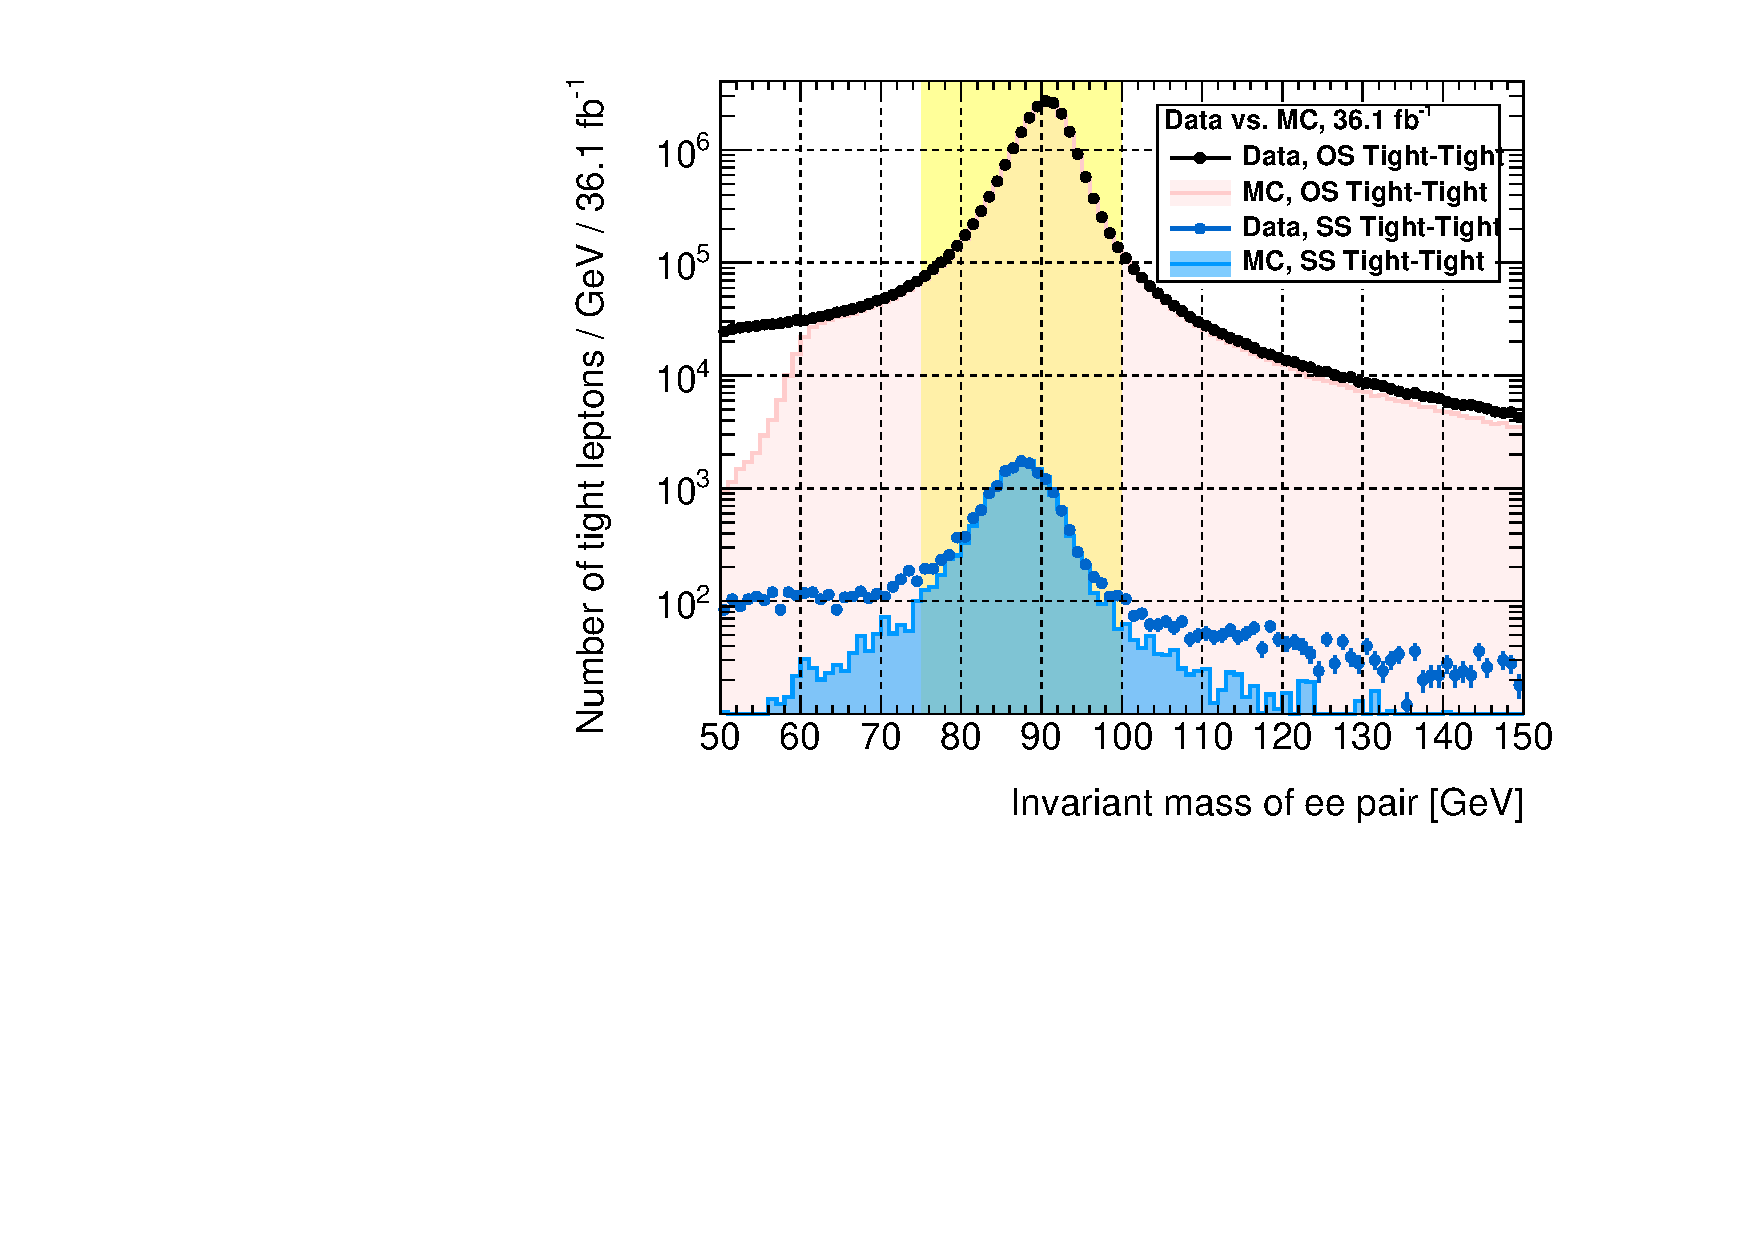
\includegraphics[width=\textwidth]{Data_vs_MC_Pass_EL}
\end{subfigure}
\begin{subfigure}[b]{0.45\textwidth}
	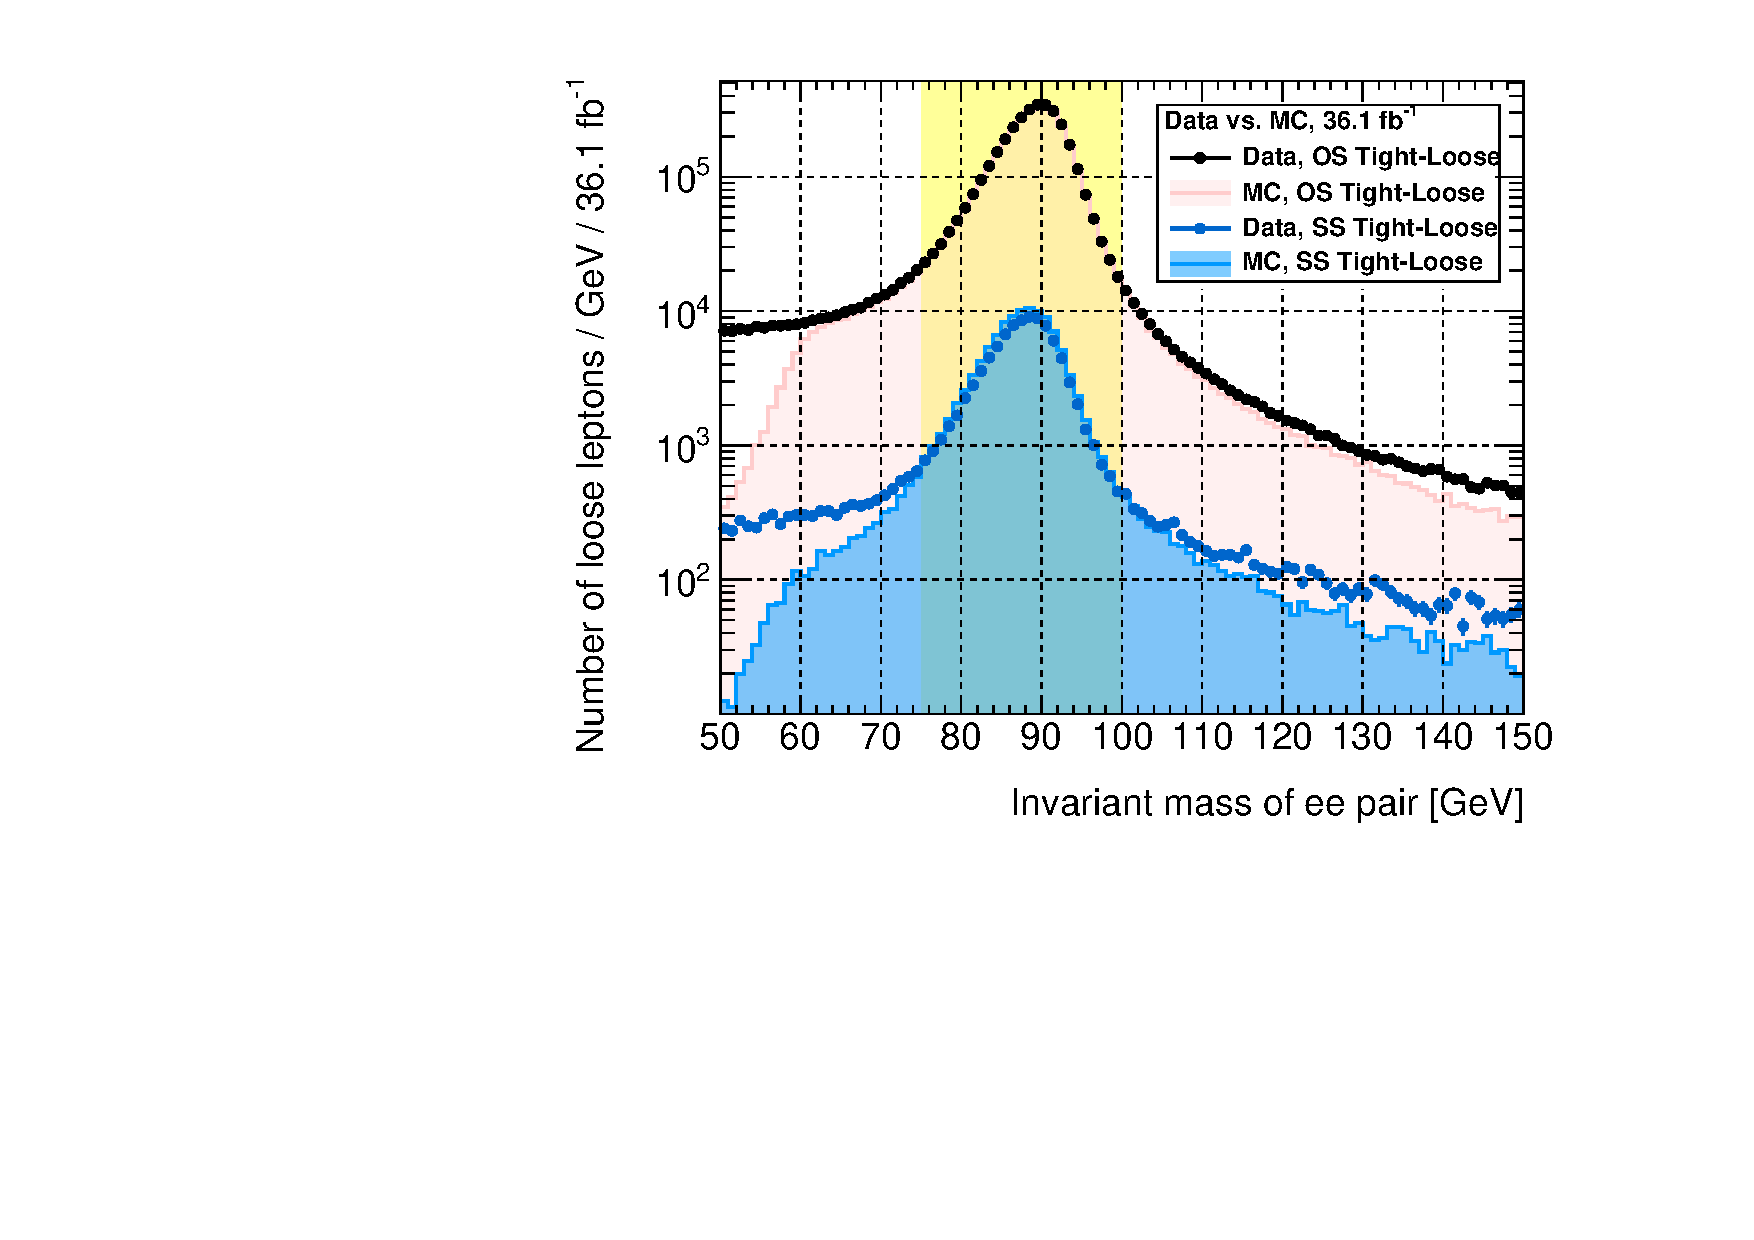
\includegraphics[width=\textwidth]{Data_vs_MC_Fail_EL}
\end{subfigure}
\caption{Invariant mass of opposite- and same-sign electron pairs, 
when both electrons satisfy signal requirements (left) or one of them fails them (right). Drell-Yan MC samples are not included, thus the drop in the MC distributions (light magenta filled area).}
\label{fig:chargeflip_mee}
\end{figure}

Charge-flip rates are measured in data relying on a clean $Z\to ee$ sample ($75<m_{ee}<100~\GeV$), 
in which the rates can be determined from the relative proportions of OS and SS electron pairs. 
Figure~\ref{fig:chargeflip_mee} illustrates this event selection. 
The rates are measured as function of $\eta$ and \pt, to follow their dependency to the distribution of material in the detector, 
the Brehmstrahlung emission rate, and the track curvature. 
Because of this binned measurements, and because the two electrons in a given pair generally have different kinematic properties, 
it has been found that the most efficient and least biased use of the available statistics 
is obtained by simultaneously extracting the rates in all bins via the maximization of the likelihood function describing the 
Poisson-expected yields of SS pairs: 

\begin{equation}
\begin{aligned}
{} & L(\{N^\text{SS,obs}_\varpi\}|\{\xi(\eta,\pt)\}) 
= \\
& \prod_{\varpi} \mathcal P\left(N^\text{SS,obs}_\varpi|w_\text{flip}(\xi(\eta_1,p_{\mathrm{T},1}),\xi(\eta_2,p_{\mathrm{T},2}))\times N^\text{OS+SS,obs}_\varpi\right)
\label{eqn:chargeflip_likelihood}
\end{aligned}
\end{equation}
with $\varpi=(\eta_1,p_{\mathrm{T},1},\eta_2,p_{\mathrm{T},2})$ indexing bins, where (arbitrarily) $p_{\mathrm{T},1}>p_{\mathrm{T},2}$; 
the expression of $w_\text{flip}$ is given by~(\ref{eqn:chargeflip_weight}). 
Statistical uncertainties on the extracted charge-flip rates are obtained (in a standard way) from the likelihood's numerically-computed Hessian matrix. 

In the nominal charge-flip measurement, the two electrons are required to satisfy signal requirements. 
To measure charge-flip rates for baseline electrons failing signal (noted $\bar\xi$ below), 
pairs with only one signal electron are used; 
this provides larger statistics than applying~(\ref{eqn:chargeflip_likelihood}) to electrons pairs where both fail the signal cuts. 
However, the expression of the likelihood has to be adapted due to the induced asymmetry between the two electrons forming the pair: 
%\small{
\begin{equation}
\begin{aligned}
{} & L(\{N^\text{SS,obs}_\varpi\}|\{\xi(\eta_1,p_{\mathrm{T},1})\},\{\bar\xi(\eta_2,p_{\mathrm{T},2})\}) 
= \\
& \prod_{\varpi} \mathcal P\left(N^\text{SS,obs}_\varpi|w_\text{flip}(\xi(\eta_1,p_{\mathrm{T},1}),\bar\xi(\eta_2,p_{\mathrm{T},2}))\times N^\text{OS+SS,obs}_\varpi\right)
\label{eqn:chargeflip_likelihood_loose}
\end{aligned}%}
\end{equation}
where this time $(\eta_1,p_{\mathrm{T},1})$ corresponds to the signal electron. 
Using the same $\eta$ and \pt binning for both measurements, 
the number of free variables in the maximization of~(\ref{eqn:chargeflip_likelihood_loose}) 
-- as well as the number of terms in the product forming $L$ -- 
is twice as large as the nominal case~(\ref{eqn:chargeflip_likelihood}). 
In fact, a by-product of the maximization of~(\ref{eqn:chargeflip_likelihood_loose}) is another determination of the charge-flip rates for signal electrons, 
although with a more limited precision than obtained in the nominal measurement~(\ref{eqn:chargeflip_likelihood}).

Background subtraction is performed through a simple linear extrapolation of the invariant mass distribution sidebands; 
it matters mostly for low \pt in the nominal measurement, 
and for the additional measurement with baseline electrons failing signal requirements, where the level of background is larger. 

\subsection*{Measured rates}
\label{subsec:chargeflip_rates}

\begin{figure}[htb!]
\centering
\begin{subfigure}[b]{0.49\textwidth}
	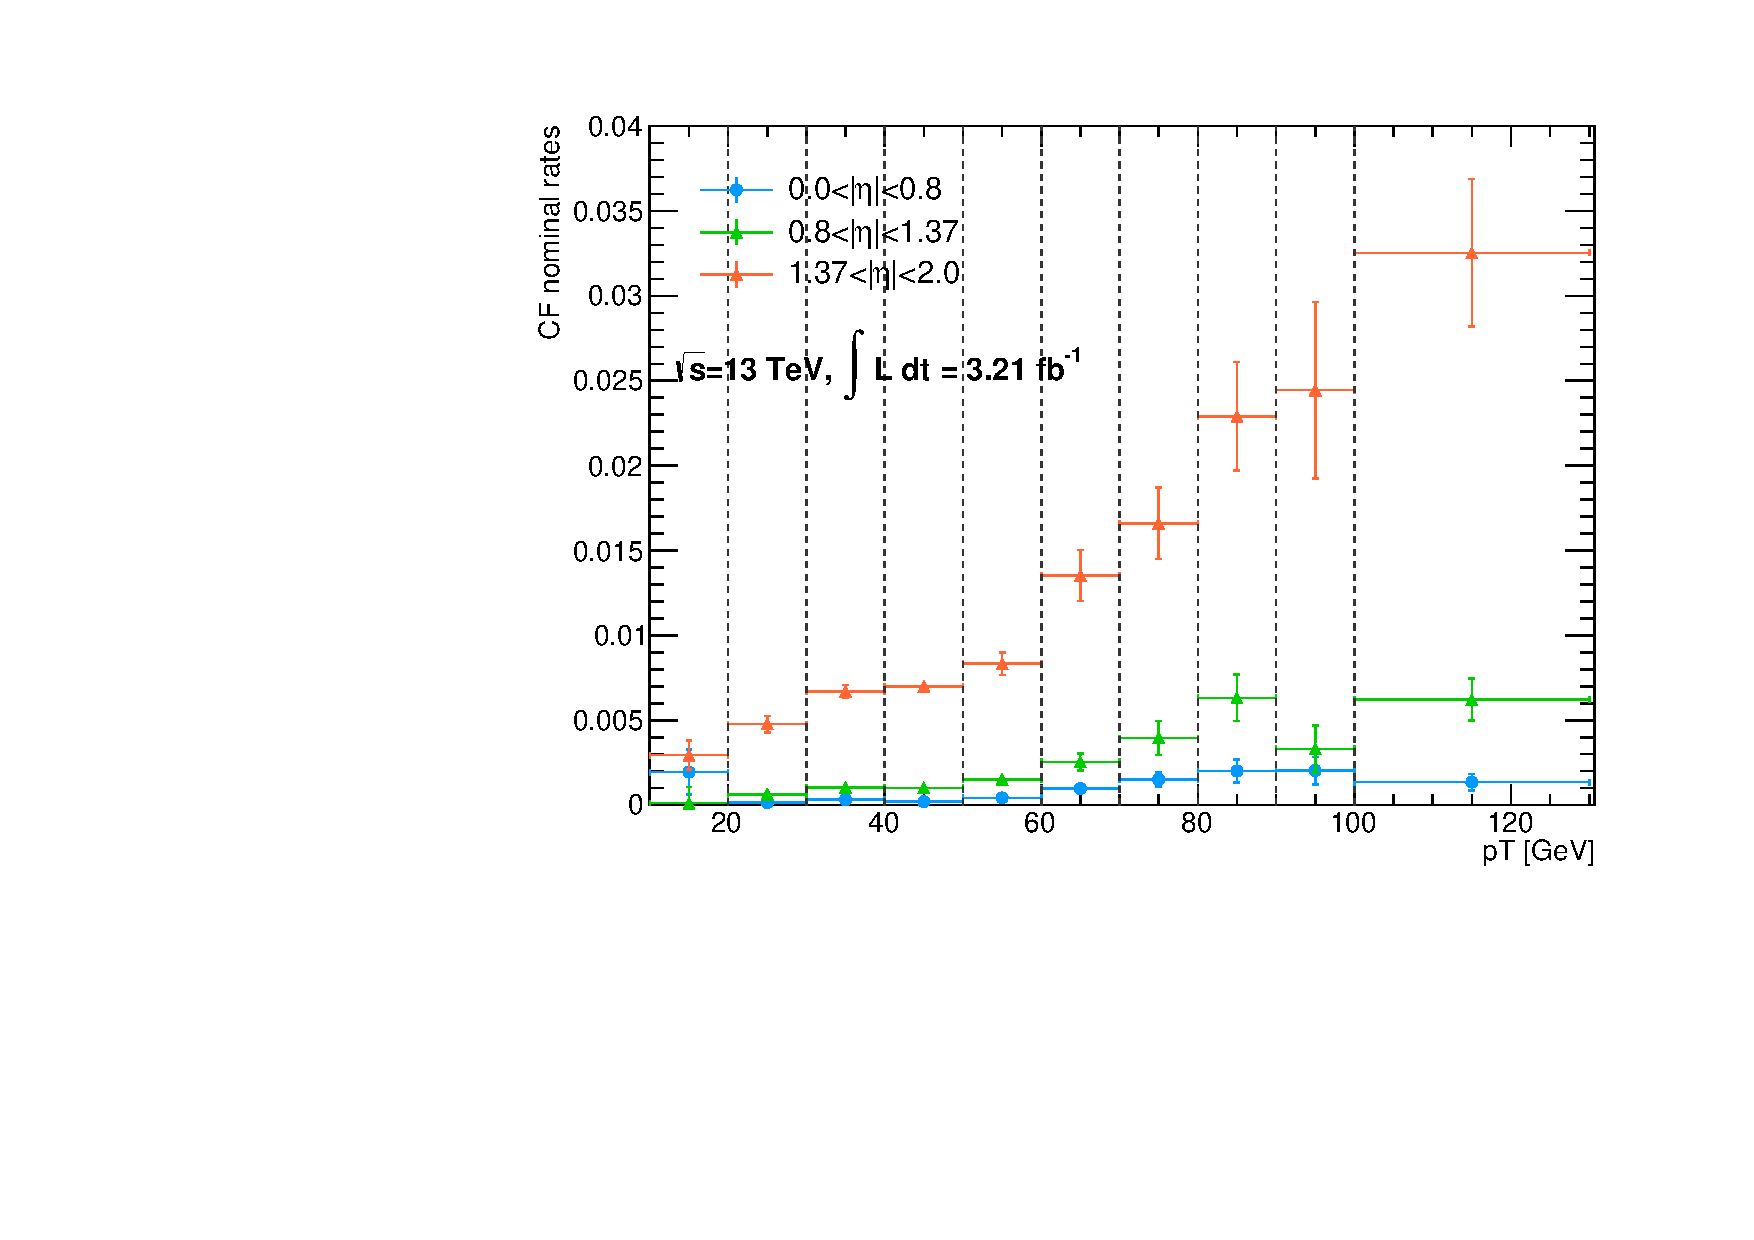
\includegraphics[width=\textwidth]{CFratesVSpt_data15}
	\caption{Data, signal electrons}\label{fig:Chflip_nominalData}
\end{subfigure}
\begin{subfigure}[b]{0.49\textwidth}
	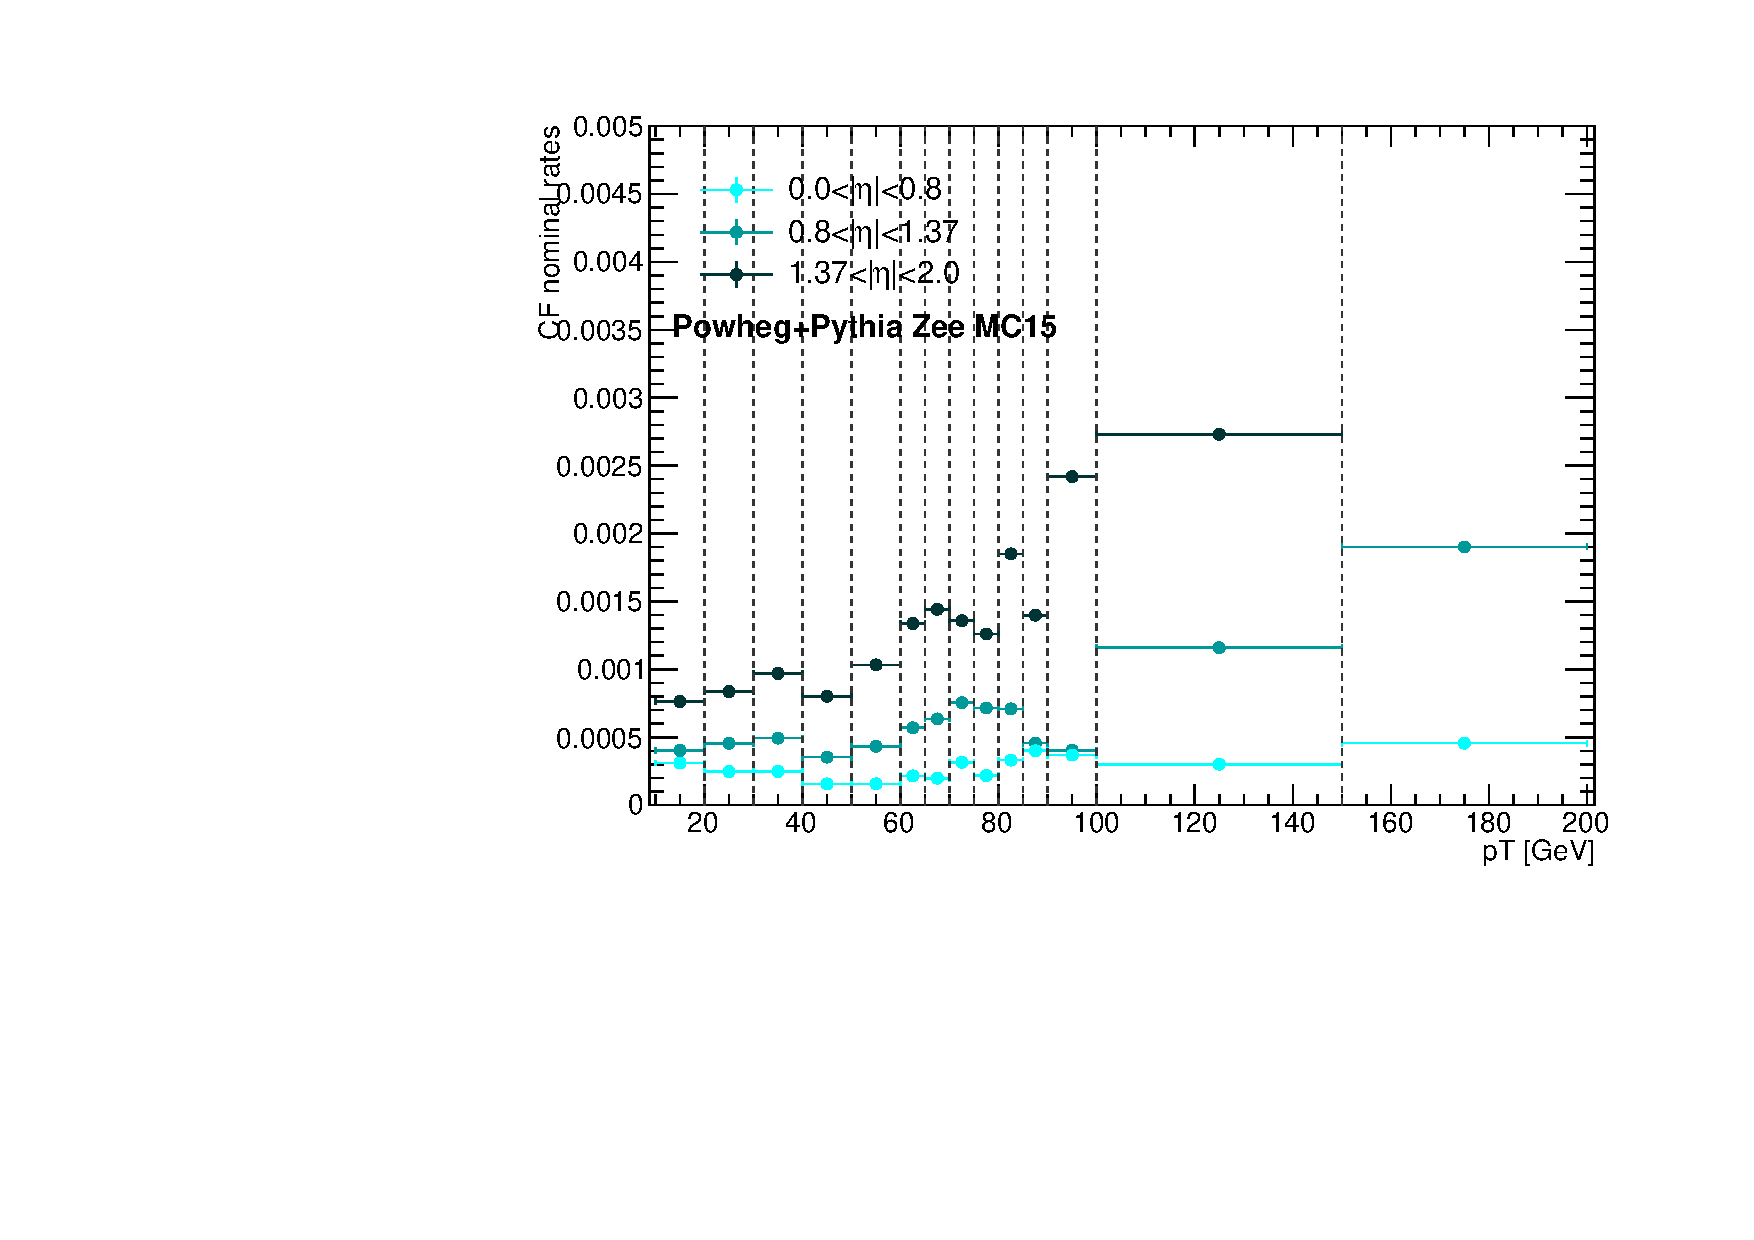
\includegraphics[width=\textwidth]{CFratesVSpt_MC15}
	\caption{MC, signal electrons}\label{fig:Chflip_nominalMC}
\end{subfigure}
\begin{subfigure}[b]{0.49\textwidth}
	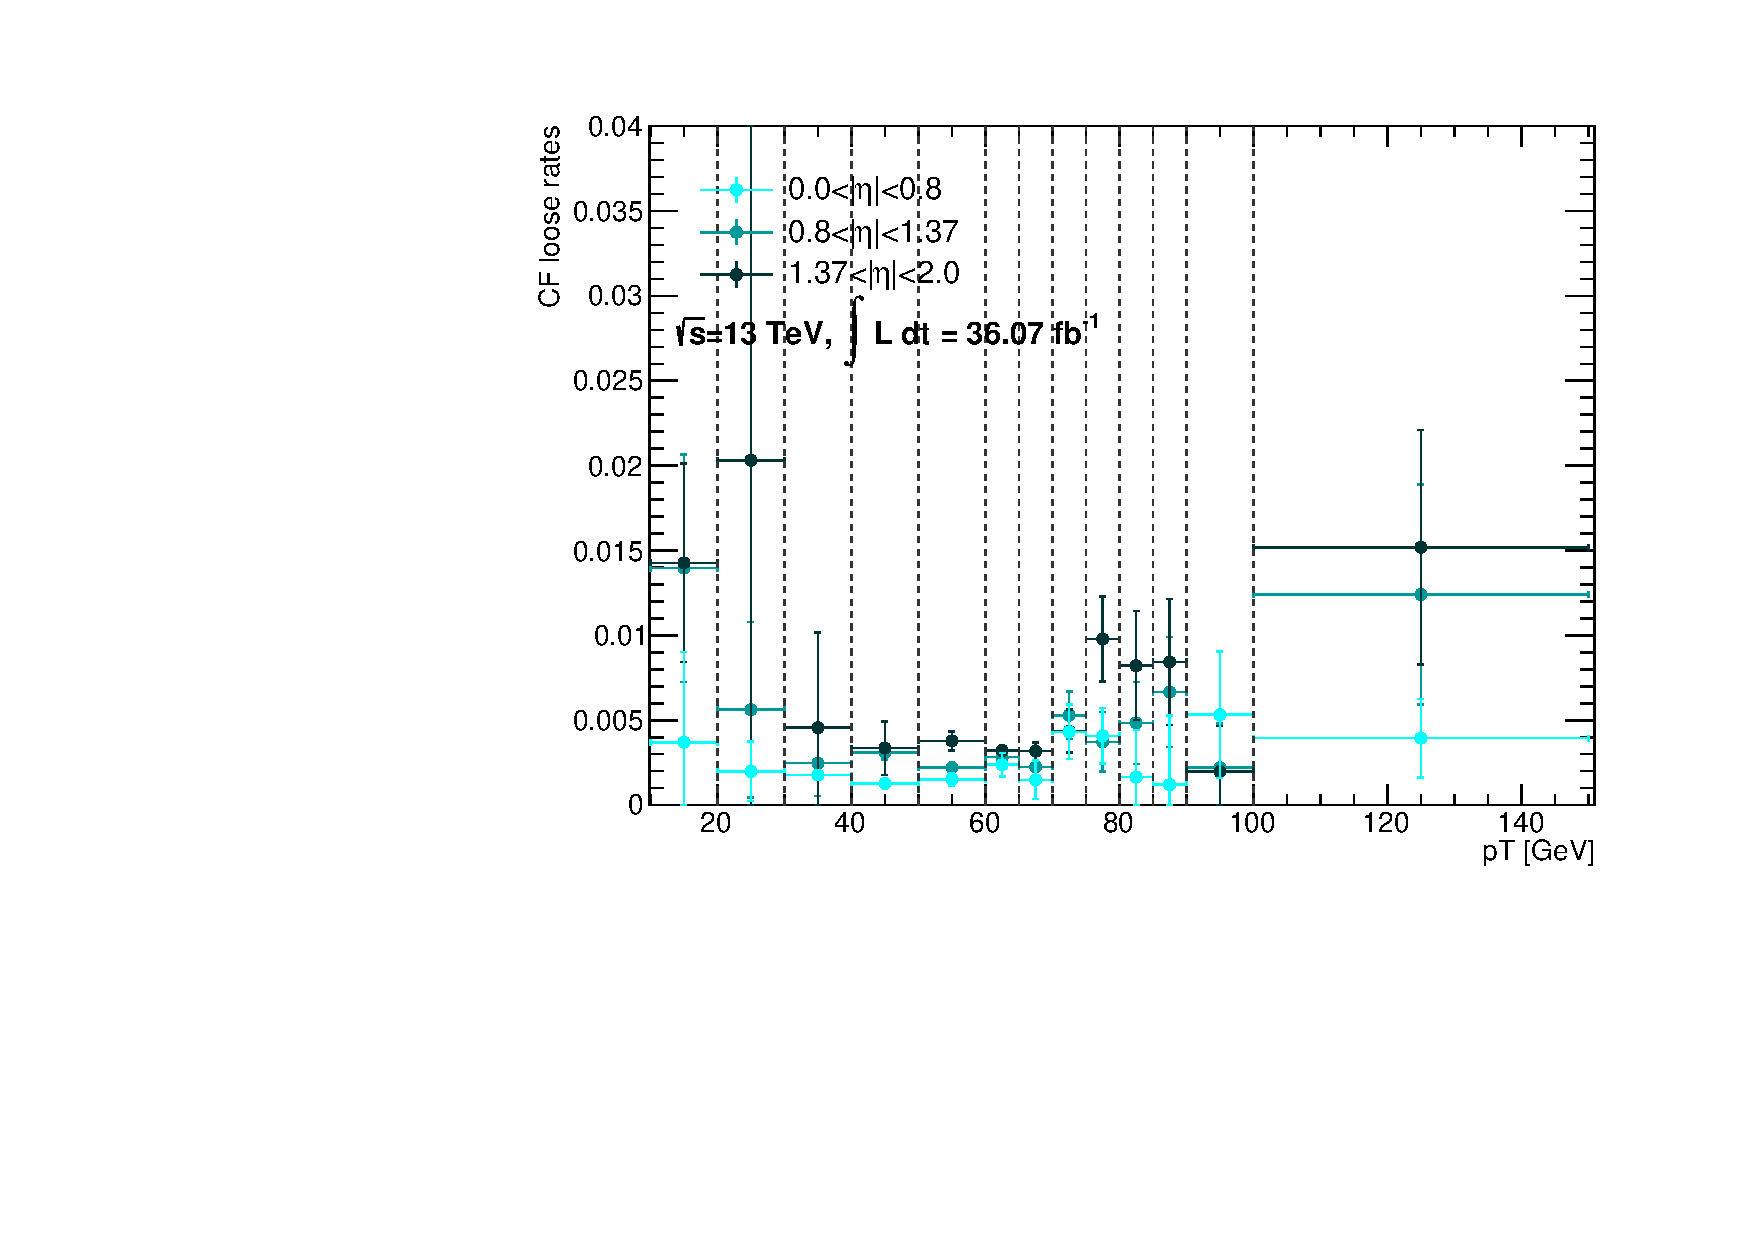
\includegraphics[width=\textwidth]{CFratesLOOSEVSpt_data15}
	\caption{Data, baseline-failing-signal}\label{fig:Chflip_looseData}
\end{subfigure}
\begin{subfigure}[b]{0.49\textwidth}
	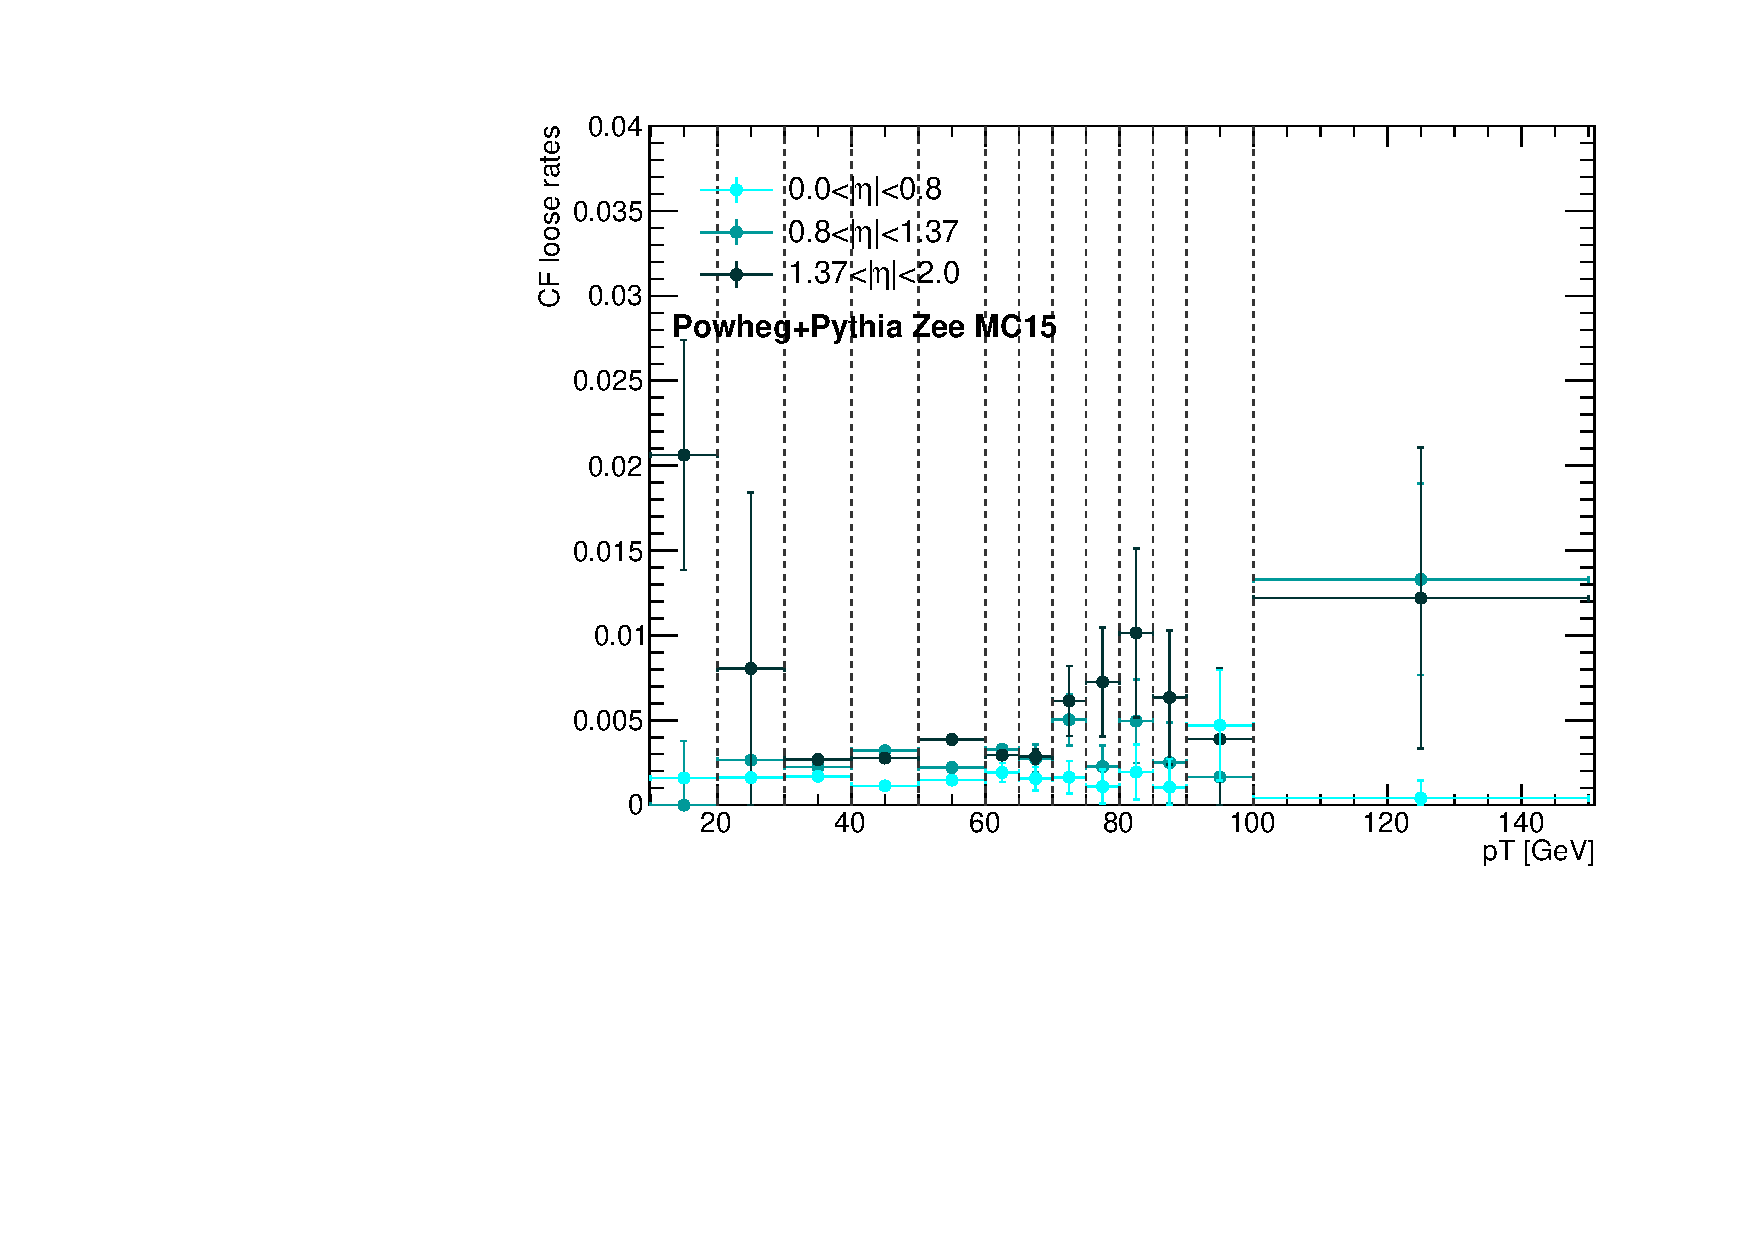
\includegraphics[width=\textwidth]{CFratesLOOSEVSpt_MC15}
	\caption{MC, baseline-failing-signal}\label{fig:Chflip_looseMC}
\end{subfigure}
\caption{Charge-flip rate as measured in data (left) and MC (right). 
Only the statistical uncertainty is displayed. The last \pt bin is inclusive.}
\label{fig:ChFlip_Rate}
\end{figure}

The charge-flip rates measured in data and MC are shown on Figure~\ref{fig:ChFlip_Rate}. 
 In data, the nominal rates (Figure~\ref{fig:Chflip_nominalData}) go up to $\sim$0.1\% in the barrel region ($|\eta| < 1.37$), 
 while it increases up to $\sim$0.2\% in the end-cap region ($|\eta > 1.37|$). 
 For baseline electrons failing signal requirements (Figure~\ref{fig:Chflip_looseData}), 
 the rates are in general greater than the nominal ones in every bin, as expected. The charge-flip rates for these electrons go up to $\sim$0.5\% in the barrel region and up 1\% in the end-cap region. Compared to the rates used in the previous version of the analysis~\cite{ATLAS-CONF-2016-037}, the central values are much lower now. After suppressing the charge flip events with the charge-flip 
electron BDT classifier described in Section~\ref{subsec:strategy.sel.obj}, 
the charge flip rates are strongly reduced for both signal and baseline-failing-signal electrons (up to a factor 20 in some bins). Figure~\ref{fig:ETA_SS_BDTEL}
illustrates the charge flip background reduction in a loose selection.
\begin{figure}[htb!]
\centering
\begin{subfigure}[t]{0.66\textwidth}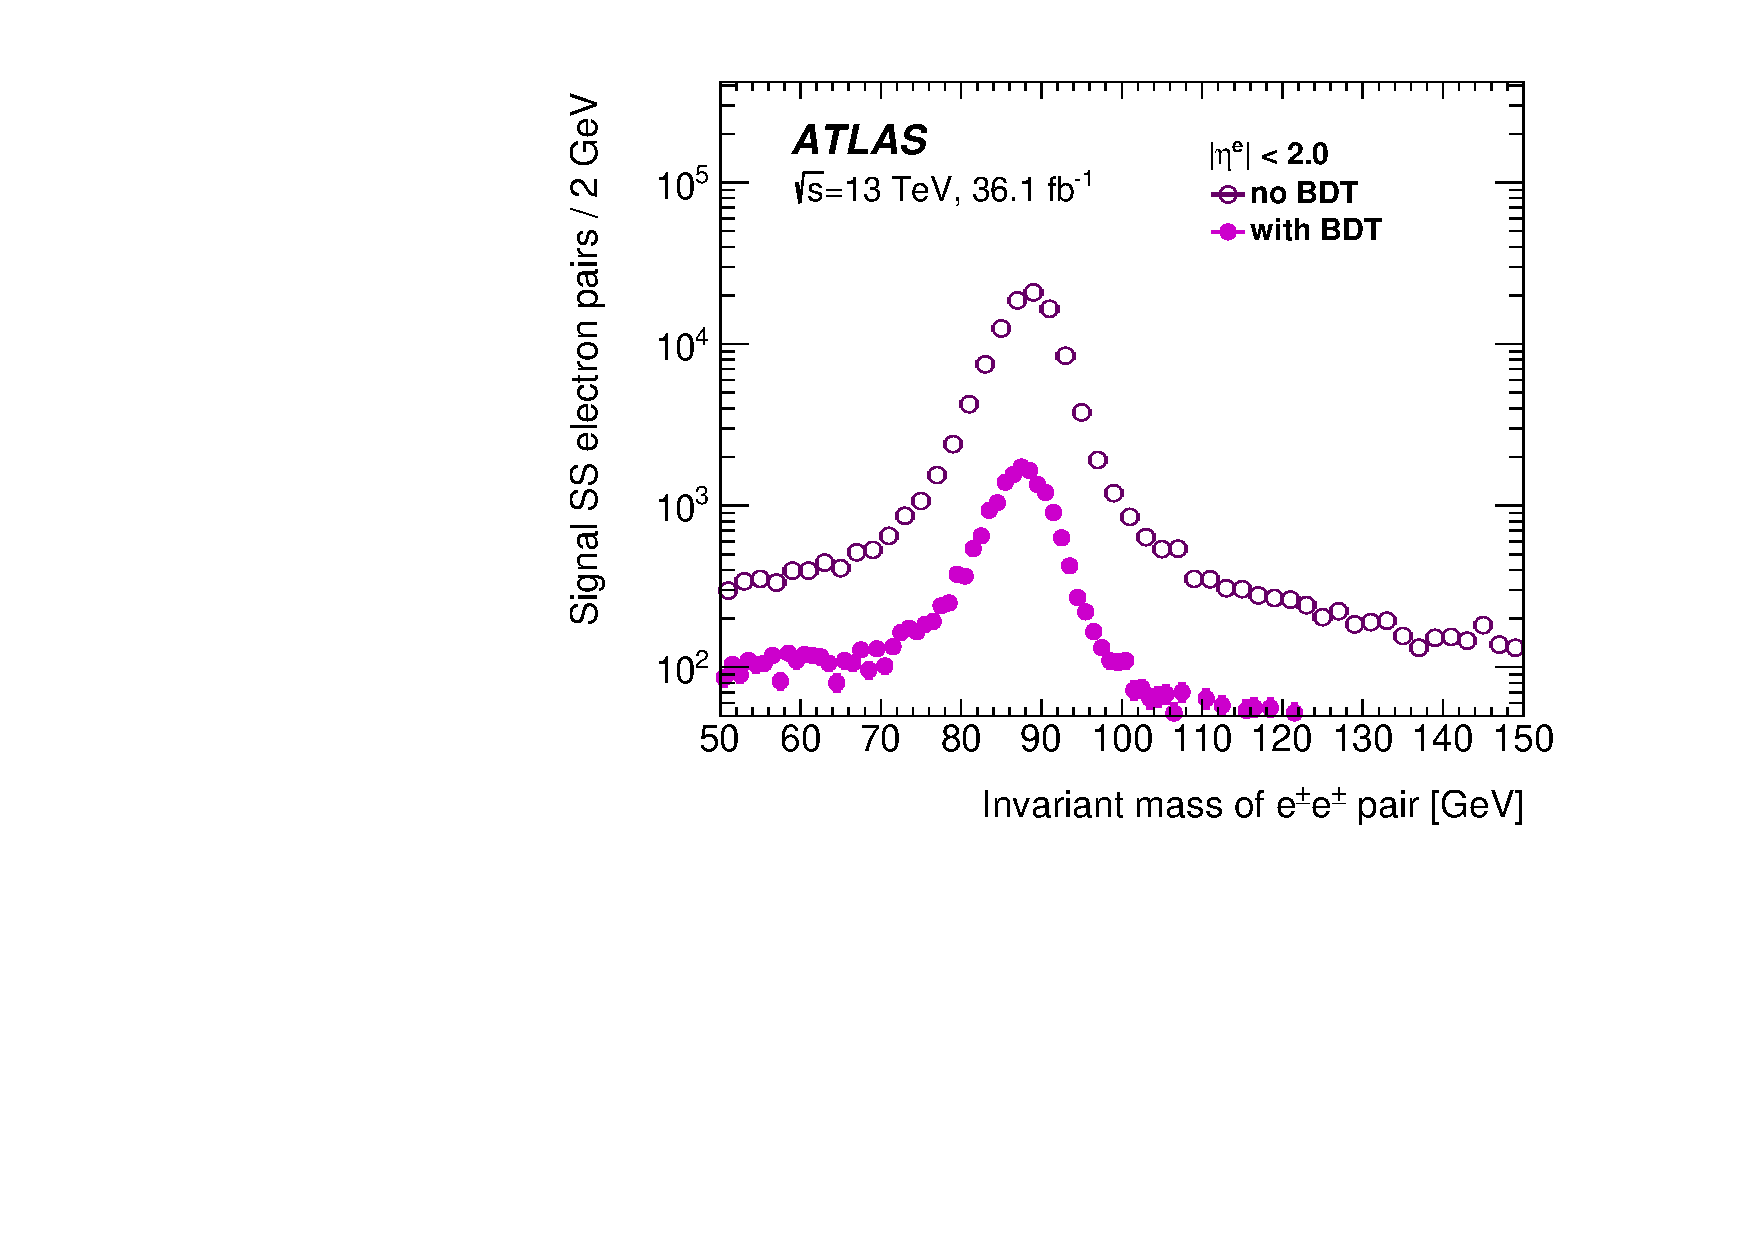
\includegraphics[width=\textwidth]{ETA_SS_BDTEL}\end{subfigure}
\caption{Invariant mass of the signal $e^{\pm} e^{\pm}$ pair distribution with (full markers) and without (open markers) charge-flip electron BDT selection applied.
}
\label{fig:ETA_SS_BDTEL}
\end{figure}
Below 30~\GeV\, the statistics are very low for the loose measurement; however, these results are used only to measure the electron fake rate and, as illustrated in Figure~\ref{Figurefakes_preselection_electron}, in this \pt interval the charge flip background is negligible.
% while the statistical uncertainties decreased significantly given the increase of up to a factor three in data luminosity. 

The charge-flip rates in MC (Figure.~\ref{fig:Chflip_nominalMC},~\ref{fig:Chflip_looseMC}) 
are obtained by applying the same methodology as in data. 
Generally, the rates are not very far from data, validating the use of MC to predict charge-flip background 
in several of the optimization studies presented in this document. 
In addition, a closure test is performed on $t\bar t$ MC, 
checking that weighted OS events can reproduce the distribution of SS charge-flip events (identified by truth-matching). 
A good overall agreement is found, largely within the assigned uncertainties
as shown in Figure~\ref{fig:ChargeFlip_ClosureTest}. 

\begin{figure}[htb!]
\centering
{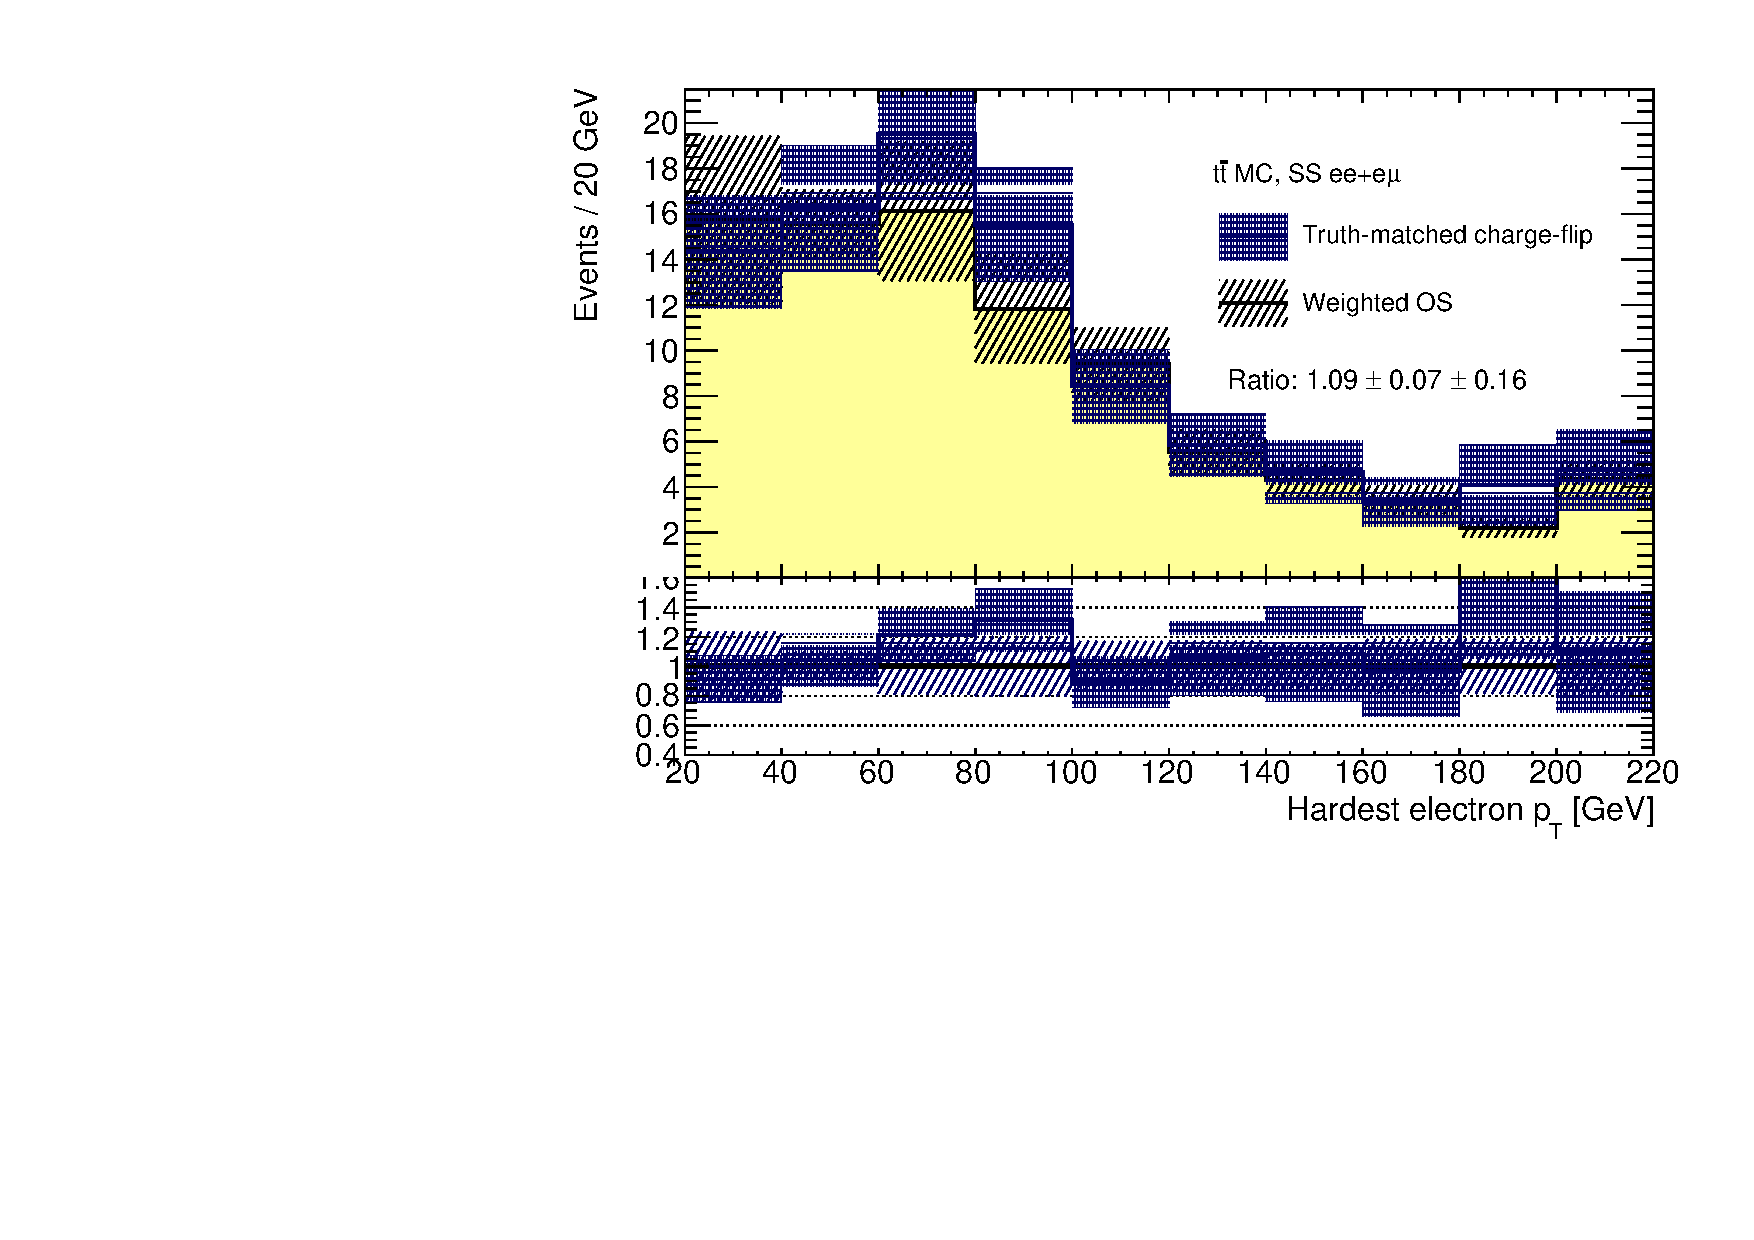
\includegraphics[width=0.49\textwidth]{Closure_HardestElectronPt}}
{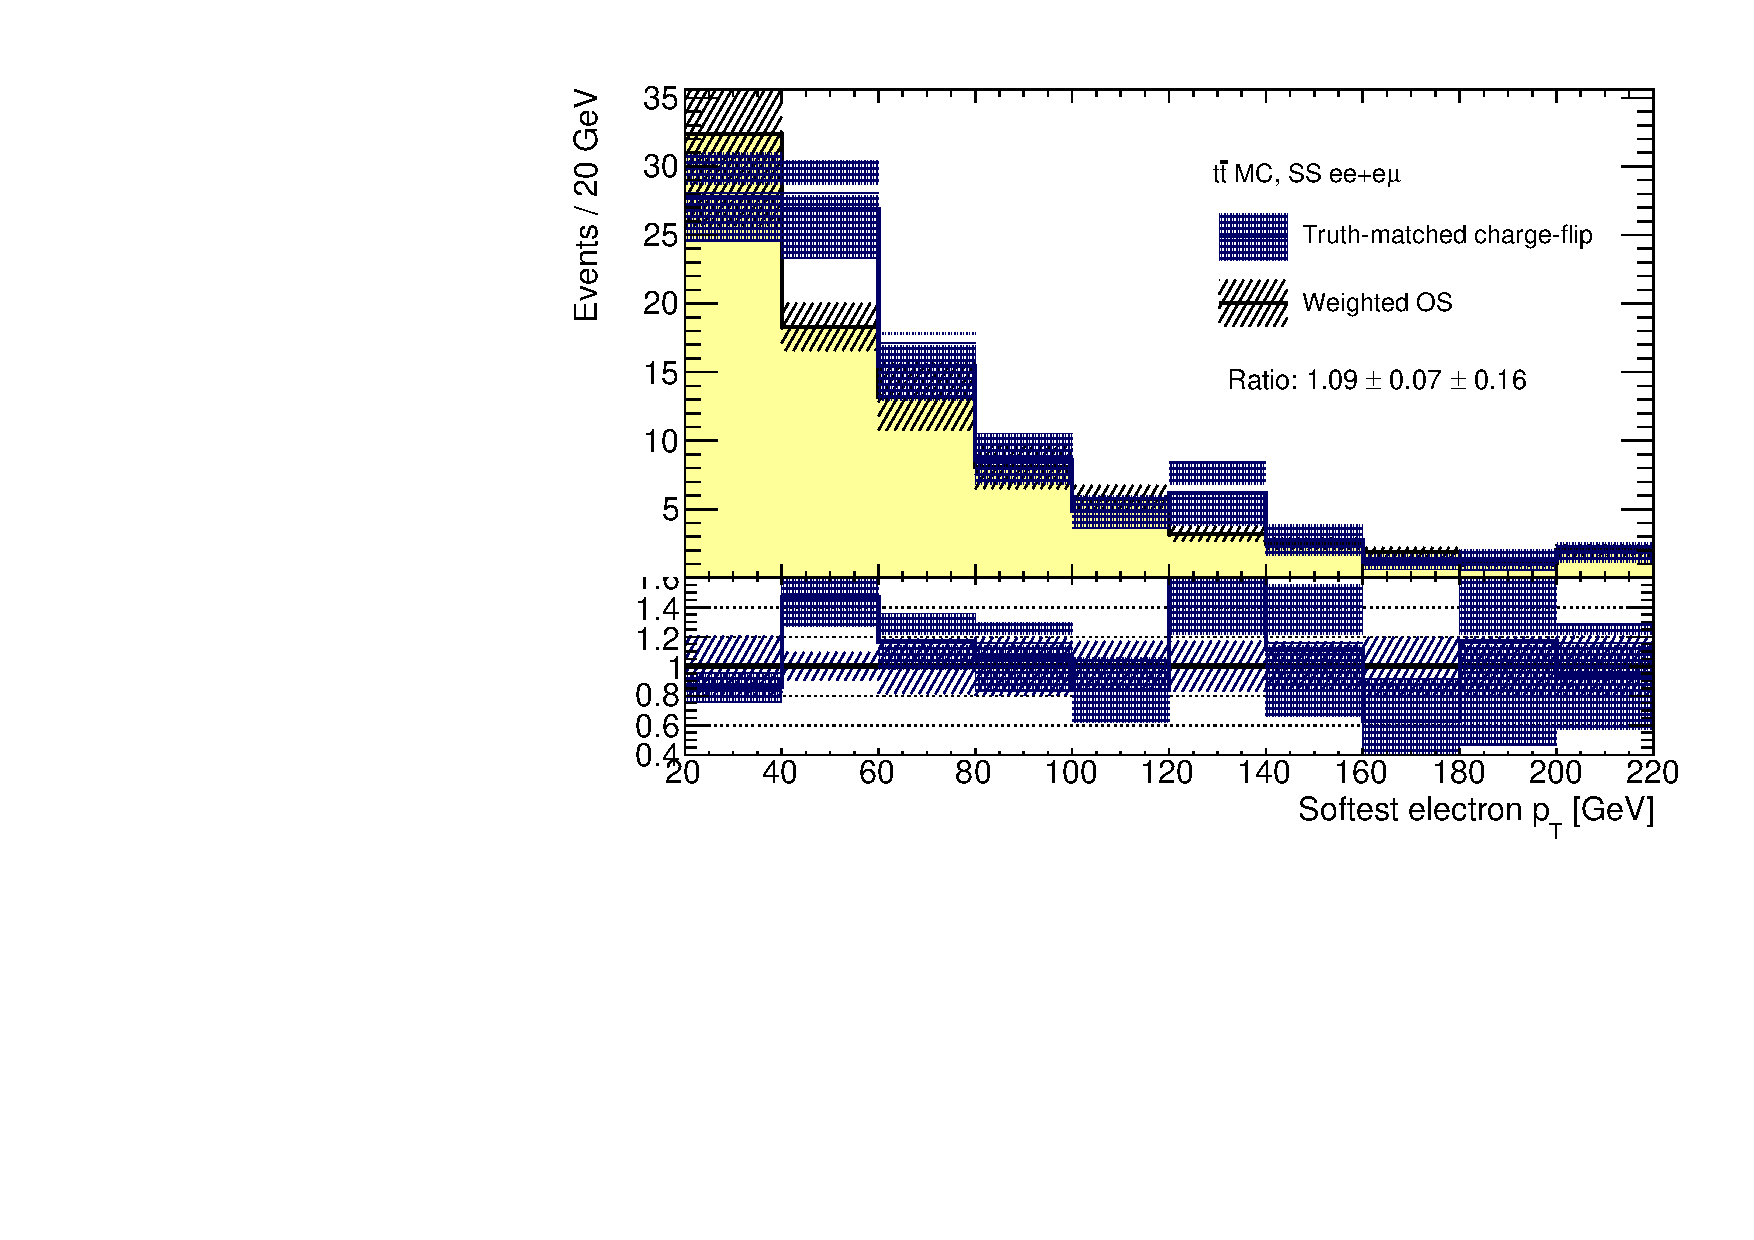
\includegraphics[width=0.49\textwidth]{Closure_SoftestElectronPt}}
{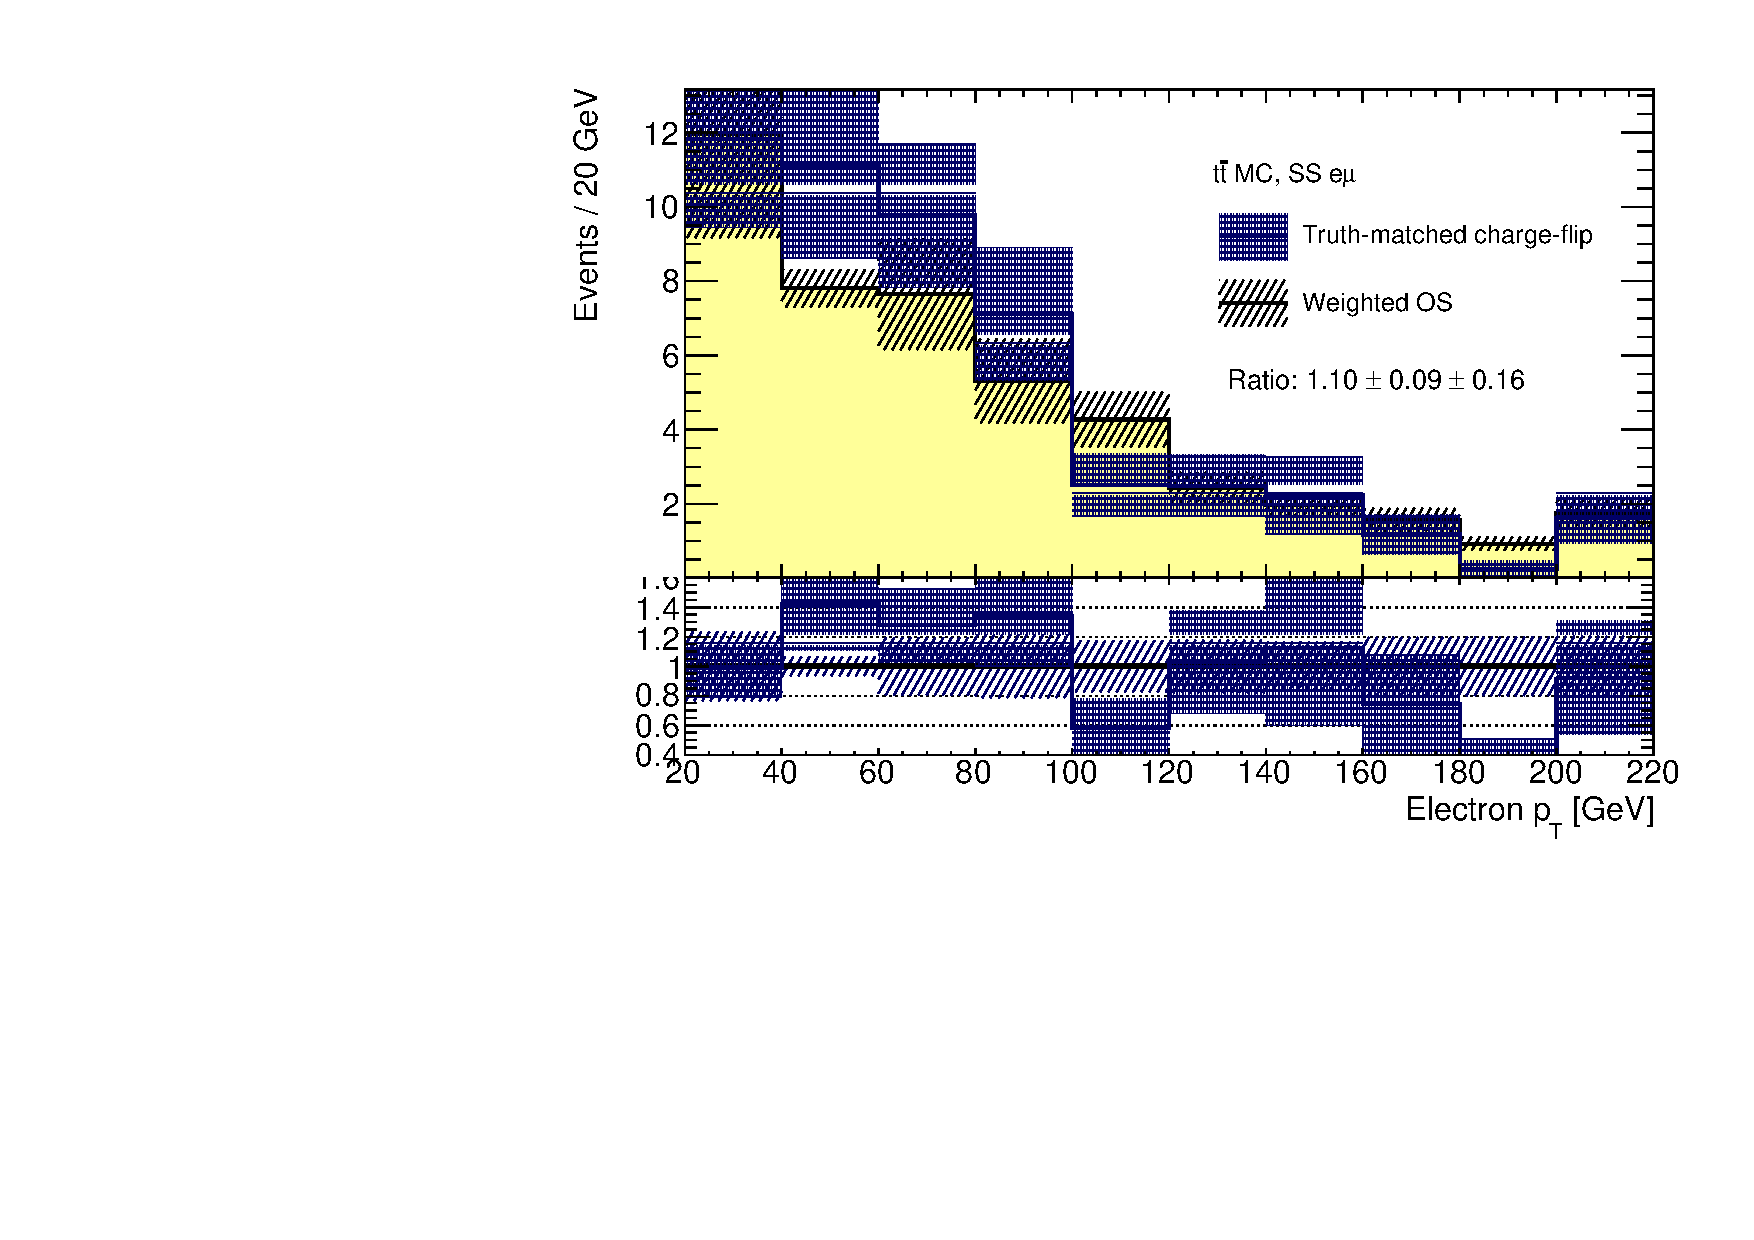
\includegraphics[width=0.49\textwidth]{Closure_EMU_ElectronPt}}
%{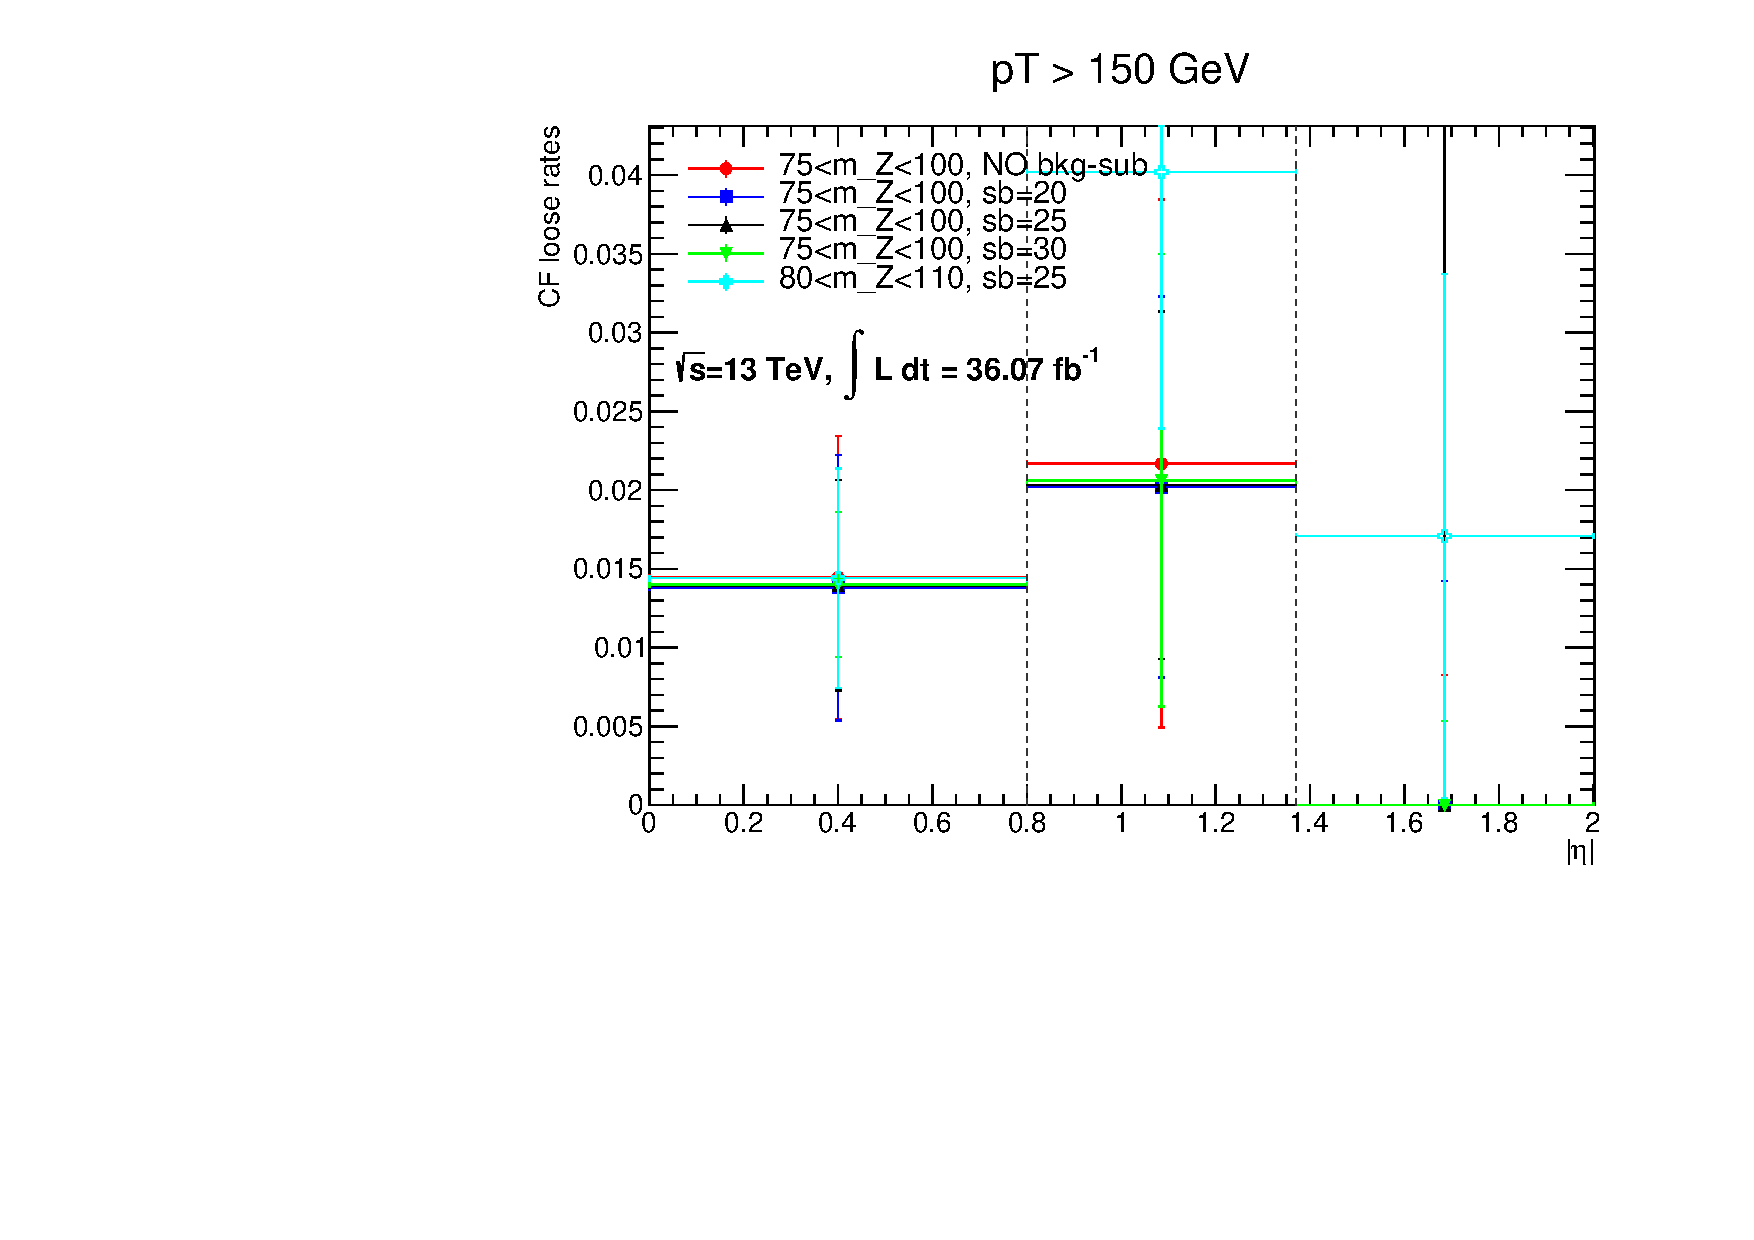
\includegraphics[width=0.49\textwidth]{CFratesLOOSE___SYStypes___PTbin13}}
\caption{Closure test for the charge-flip background prediction, for simulated $t\bar t$ events 
using charge-flip rates measured in $Z\to ee$ MC 
(with the systematic uncertainties from the data measurements, though). 
Events are selected in the $e\mu$ and $ee$ channels, using signal leptons only, 
and charge-flipped electrons are identified by truth-matching. 
}
\label{fig:ChargeFlip_ClosureTest}
\end{figure}

\subsection*{Systematic uncertainties}
\label{subsec:chargeflip_uncertainties}

%% \begin{figure}[t!]
%% \centering
%% \begin{tabular}{rr}
%% \begin{subfigure}[b]{0.5\textwidth}
%% 	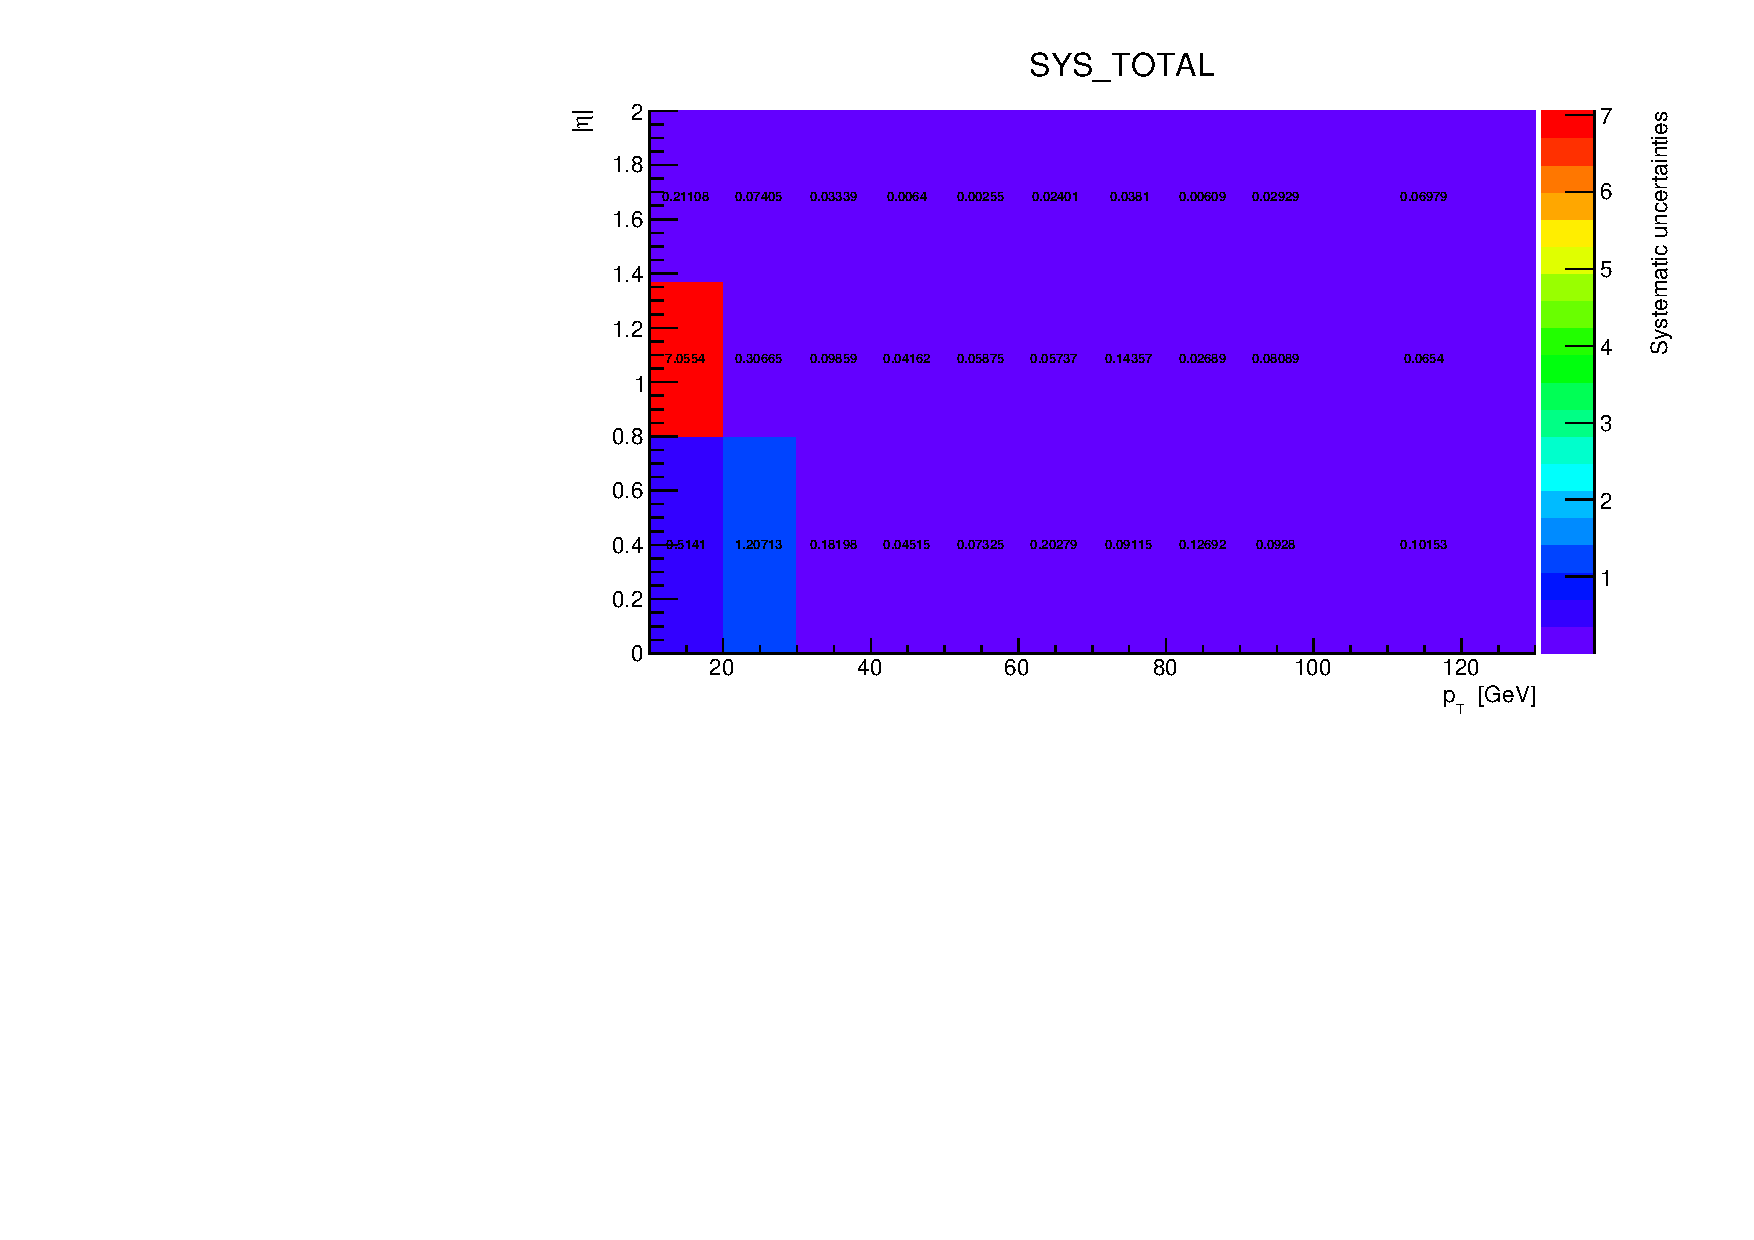
\includegraphics[width=\textwidth]{2D_histo_SYS_TOTAL}\caption{}\label{fig:bkg.chargeflip.2D_histo_SYS_TOTAL}
%% \end{subfigure} &
%% \begin{subfigure}[b]{0.5\textwidth}
%% 	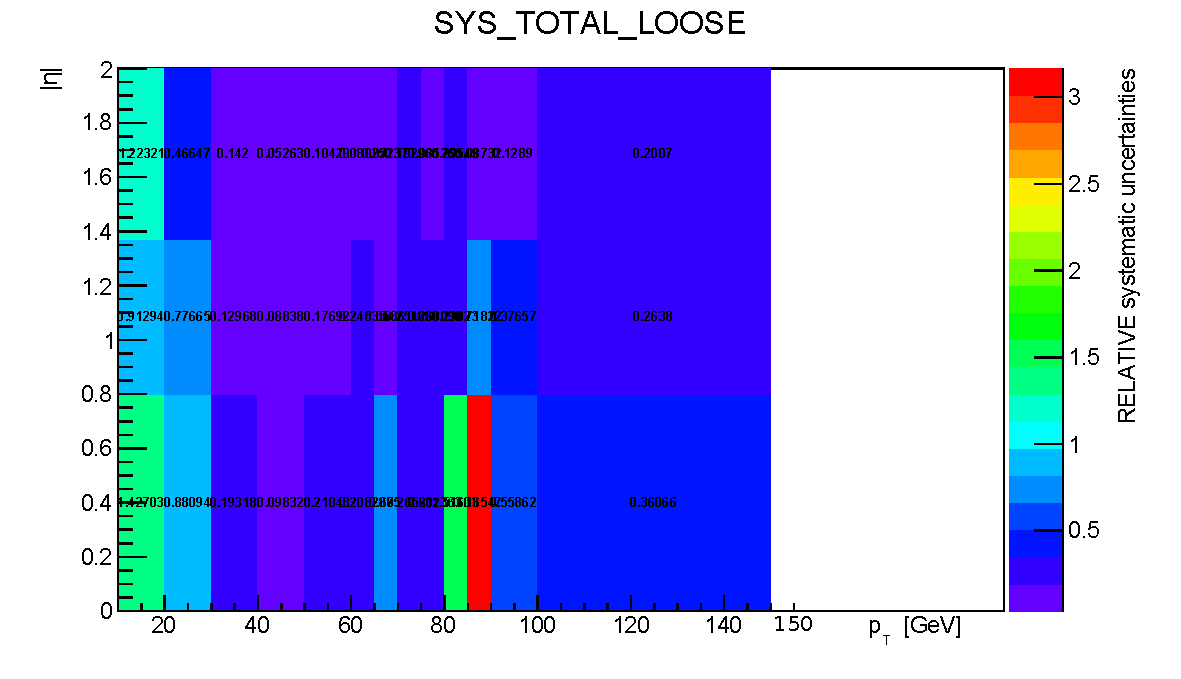
\includegraphics[width=\textwidth]{2D_histo_SYS_TOTAL_LOOSE}\caption{}\label{fig:bkg.chargeflip.2D_histo_SYS_TOTAL_LOOSE}
%% \end{subfigure}
%% \end{tabular}
%% \caption{Total systematic uncertainties on the charge-flip rates for electrons satisfying the signal requirements (\ref{fig:bkg.chargeflip.2D_histo_SYS_TOTAL}),
%% and for baseline electrons failing the signal requirements (\ref{fig:bkg.chargeflip.2D_histo_SYS_TOTAL_LOOSE}). 
%% }
%% \label{fig:ChFlip_SYS_Total}
%% \end{figure}

The main uncertainties on the measured charge-flip rates come from the presence of background and the way it is estimated. To assess them, variations of the selection and background estimation are considered: 
\begin{itemize}
\item[1)] $75<m_{ee}<100~\GeV$, no background subtraction;
\item[2)] $75<m_{ee}<100~\GeV$, sidebands of 20~\GeV;
\item[3)] $75<m_{ee}<100~\GeV$, sidebands of 25~\GeV~(nominal measurement);
\item[4)] $75<m_{ee}<100~\GeV$, sidebands of 30~\GeV;
\item[5)] $80<m_{ee}<100~\GeV$, sidebands of 20~\GeV.
\end{itemize}

The effect of applying the background subtraction itself is evaluated by comparing configurations 1 and 3. 
The impact of the width of the $m_{ee}$ chosen for the measurement is  by comparing configurations 3 and 5, 
while the sideband width effects are evaluated by comparing configuration 3 and 2, or 3 and 4. 
The largest deviation in each bin is taken as the systematic uncertainty on the charge-flip rate.

%The resulting systematic uncertainties on the charge-flip rates are presented in Figure~\ref{fig:ChFlip_SYS_Total}. 

For the signal electrons charge-flip rates the systematic uncertainties vary in general between 2\% and 20\% (increasing up to $>50\%$ in the region with $\pt < 10~\GeV$), whereas for baseline-failing-signal electrons they vary between 3\% and 30\% (increasing up to $>50\%$ in the region with $\pt < 10~\GeV$). Part of these large values, at low \pt and in the [80,90]~\GeV~\pt interval, can be explained by large statistical fluctuations between the different configurations.
